\documentclass[2pt,twocolumn]{article}
\usepackage[english,russian]{babel}
\usepackage{multicol}
\usepackage{geometry}
\usepackage{longtable}
\usepackage{graphicx}
\usepackage[table,xcdraw]{xcolor}
\usepackage{setspace}
\usepackage{aligned-overset}
\onehalfspacing
\newcommand\tab[1][1cm]{\hspace*{#1}}
\geometry{
  a4paper,
  top=25mm, 
  right=15mm, 
  bottom=25mm, 
  left=15mm
}
\title{Something}
\author{Someone}

\begin{document}
\setcounter{page}{43}
\begin{flushleft}
    \tab 2. $t = \frac{\mu\rho V}{RTM} = 8.35\cdot 10^{-3}$ с\\
    \tab 3. Выделим участок поверхности шара единичной площади и найдем силу, действующую на выделенный участок. Напряженность электрического поля у поверхности шара снаружи равна $\overset{\rightarrow}{|E|}=\frac{Q}{4\pi\varepsilon_0 R^2}$,
    а внутри -- $\overset{\rightarrow}{|E_{\text{вн}}|}=0.$ Пусть $\overset{\rightarrow}{E'}$ -- напряженность поля, создаваемого единичной поверхностью, а $\overset{\rightarrow}{E''}$ --  напряженность поля, вблизи выделенного участка. Используя
    принцип суперпозиции, для поля над участком и под ним (внутри сферы) получим:\\
    \tab$\overset{\rightarrow}{|E'|} + \overset{\rightarrow}{|E''|} =\overset{\rightarrow}{|E|},~ \overset{\rightarrow}{|E'|} + \overset{\rightarrow}{|E''|} =0.$\\
    Отсюда находим напряженность поля, действующего на выделенный участок: $\overset{\rightarrow}{|E''|}=\frac{\overset{\rightarrow}{|E|}}{2}.$ Тогда сила, действующая на единицу площади поверхности, равна\\
    \tab$\overset{\rightarrow}{|F|}=\overset{\rightarrow}{|E''|}\frac{Q}{4\pi R^2}=\frac{Q^2}{32\pi^2\varepsilon_0 R^4}.$\\
    Направлена эта сила по радиусу от центра шара. Теперь запишем условие равновесия для половинки шара непосредственно пере разрывом:\\
    \tab $\overset{\rightarrow}{|F|}\pi R^2 = 2\pi R \Delta R \sigma_{\text{вн}}$\\
    Отсюда найдём величину заряда Q:
    \tab$Q=8\pi R \sqrt{\varepsilon_0 R \Delta R \sigma_{\text{пр}}}\approx 2\cdot 10^{-2}$ Кл.\\
    \tab 4. $F = ^3/_4 l = 9$см.\\
    \textbf{<<Квант>> для младших школьников}\\
    (см. <<Квант>> № 2, с. 45)\\
    \tab 1. Перепишем зашифрованный ребус в столбик:\\
    \begin{table}[h]
        \begingroup
    \fontsize{6pt}{8pt}\selectfont
        \begin{tabular}{ll}
          & ТАМТАМ \\
        + & МРАК   \\ \hline
          & КОШМАР
        \end{tabular}%
    \endgroup
    \end{table}
    Нетрудно сообразить, что $A = 9$, $O = 0$ так что\\
    \tab \tab $M+K=P+10$\\
    \tab \tab$K = T+1$\\
    и либо $T+P+1=M$, либо $T+P+1=M+10.$\\
    \tab Пусть сначала $T+P+1=M.$ В этом случае $T=4$, $K=5$, так что
    \tab \tab $\left\{
        \begin{array}{ccc}
          M+5=P+10, \\
          P+5=M. \\
        \end{array}
      \right.$\\
    \tab Учитывая, что $1\leq P \leq 9,~1\leq M\leq 9,$ получаем три возможности для P и М: $P=1,~2,~3$ 
    и, соответственно, $1\leq M \leq 9.$\\
    \tab   При $P=1$ и $P=3$ получаем две расшифровки:\\
    \begin{table}[h]
        \begingroup
    \fontsize{7pt}{9pt}\selectfont
        \begin{tabular}{lrllr}
          & $496~496$ &   &   & $498~498$ \\
        + & $6~195$   & и & + & $8~395$   \\ \cline{2-2} \cline{5-5} 
          & $502~691$ &   &   & $506~893$
        \end{tabular}%
        \endgroup
    \end{table}
    а при $P=2$ получаем $\text{Ш} = 4 = \text{T}$, что невозможно.\\
    \tab Для случая, когда $\text{Т}+\text{P}+1=M+10,$ получаем $\text{T}=9=\text{A},$ что также не годится.\\
    \begin{figure}[h!]
        \center{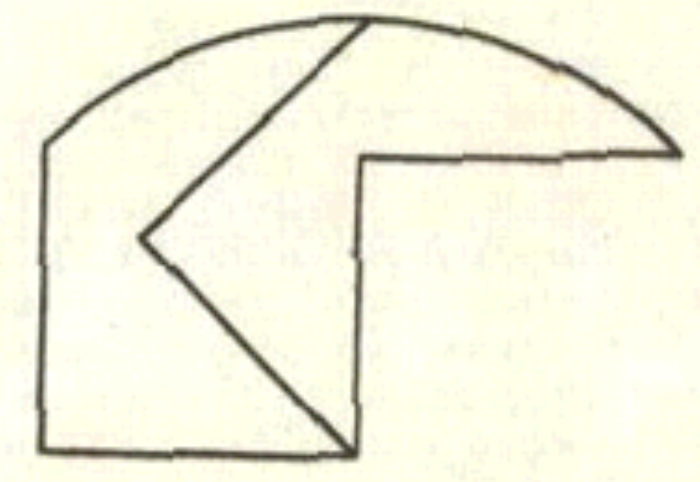
\includegraphics[scale=0.3]{image.png}}\\
        {\small Рис. 8.}
    \end{figure}
    \tab Итак, существует ровно две различные расшифровки ребуса. В условии говорится, что знатоков было несколько -- значит, их двое!\\
    \tab 3. См. рисунок 8.\\
    \tab 4. Переверём стаканы шесть раз, каждый раз оставляя неперевернутым новый стакан. Тогда каждый стакан окажется перевернутым пять раз, то есть все стаканы будут поставлены вверх дном.\\
    \tab 5. Точки, стоящие на одной вертикали, нельзя красить все в один цвет (иначе можно будет построить несколько прямоугольников с одноцветными вершинами).Поэтому на каждой вертикали должны быть точки обоим цветов. Очевидно, что если найдутся две вертикали с одинаковым расположением одноцветных точек, то найдется и прямоугольник с одноцветными вершинами. Из трех разноцветных точек, стоящих на одной вертикали, две точки обязательно одинакового цвета. Две же одноцветные точки вертикали могут занимать только три разных положения(см. рисунок 9)\\
    \begin{figure}[h!]
        \center{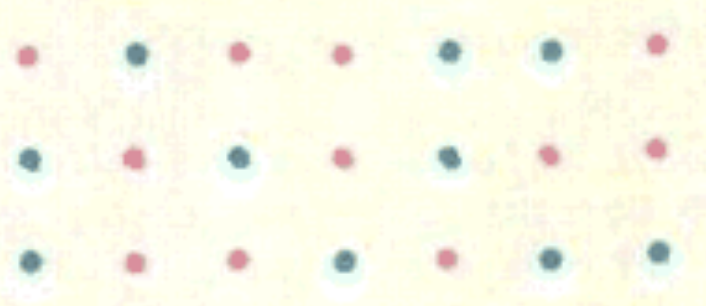
\includegraphics[scale=0.3]{image2.png}}\\
        {\small Рис. 9.}
        \label{fig:image}
    \end{figure}
    красные точки на второй, третьей и четвертой вертикалях). Так как у нас имеются две цвета, то <<разных>> вертикалей может быть только шесть. Следовательно, среди имеющихся семи вертикалей по крайней мере две будут с одинаковым расположением одноцветных точек.\\
    \textbf{...и фокус не удался}\\
    \tab(см. <<Квант>> № 2, с. 47)\\
    \tab Обозначим через $\overline{a_n a_{n-1}...a_2a_1a_0}$ десятичную запись натурального числа, у которого $a_0$ единиц, $a_1$ десятков, $a_2$ сотен,...\\
    \tab Имеем:\\
    \begingroup
    \fontsize{3pt}{7pt}\selectfont
    $\overline{a_na_{n-1}...a_2a_1a_0}=10^n\cdot a_n+10^{n-1}\cdot a_{n-1}+...+10^2 \cdot a_2+10\cdot a_1+a_0=9(\overline{\underbrace{11...11}_n})\times a_n+\overline{\underbrace{11...11}_n}\cdot a_{n-1}+...+11\cdot a_2+a_1)+(a_n+a_{n-1}+...+a_3+a_2+a_1+a_0)$\\
    \endgroup
    \tab Отсюда видно, что остаток от деления числа на
\end{flushleft}
\end{document}